%%%%%%%%%%%%%%%%%%%%%%%%%%%%%%%%%%%%%%%%%
% Beamer Presentation
% LaTeX Template
% Version 1.0 (10/11/12)
%
% This template has been downloaded from:
% http://www.LaTeXTemplates.com
%
% License:
% CC BY-NC-SA 3.0 (http://creativecommons.org/licenses/by-nc-sa/3.0/)
%
%%%%%%%%%%%%%%%%%%%%%%%%%%%%%%%%%%%%%%%%%

%----------------------------------------------------------------------------------------
%	PACKAGES AND THEMES
%----------------------------------------------------------------------------------------

\documentclass[fleqn]{beamer}
\mode<presentation> {
\usepackage{threeparttable}
\RequirePackage{siunitx}
\usepackage{tabulary}
\usepackage{float}
\usepackage{graphicx}
\usepackage{subfig}
\newcommand{\wmi}{\ensuremath{W_{b_m}\left(\frac{x-Y_{t_i}}{b_m}\right) }\xspace}
\newcommand{\wmj}{\ensuremath{W_{b_m}(({x-Y_{t_i}})/{b_m}) }\xspace}
\newcommand{\kmj}{\ensuremath{K(({x-X_{t_i}})/{b_m}) }\xspace}
\newcommand{\kmi}{\ensuremath{K\left(\frac{X_{t_i} - x}{b_m}\right) }\xspace}
\newcommand{\Xtm}{\ensuremath{X_{t-}}\xspace}
\newcommand{\sbm}{\ensuremath{W}\xspace}
\newcommand{\etn}{\ensuremath{\varepsilon_i^{T_n}}\xspace}
\newcommand{\Wbn}{\ensuremath{W_{b_n}}\xspace}
\newcommand{\ms}{\ensuremath{m^*}\xspace}
\newcommand{\Rs}{\ensuremath{R^*}\xspace}
\newcommand{\lw}{\ensuremath{{L}^W_n(x, T)}\xspace}
\newcommand{\lk}{\ensuremath{{L}^K_n(x, T)}\xspace}
\newcommand{\iid}{i.i.d\xspace}
\newcommand{\ito}{It\^o\xspace}
\newcommand{\lbm}{\ensuremath{(\triangle_m\ln(1/\triangle_m))}\xspace}
\newcommand{\lbn}{\ensuremath{(\triangle_n\ln(1/\triangle_n))}\xspace}
\renewcommand{\i}{\mathrm{i}} 
\newcommand{\sumn}{\ensuremath{\sum_{k \in \nats}}\xspace}
\newcommand{\sumin}{\ensuremath{\sum_{i = 0}^{n-1}}\xspace}
\newcommand{\sumi}{\ensuremath{\sum_{k \in \ints}}\xspace}
\newcommand{\sumt}{\ensuremath{\sum_{(h,k) \in \Theta_n}}\xspace}
\newcommand{\sv}{\ensuremath{\sigma^2}\xspace}
\newcommand{\bsv}{\ensuremath{\bar{\sigma}^2}\xspace}
\newcommand{\svnt}{\ensuremath{\sigma^2}\xspace}
\newcommand{\svhk}{\ensuremath{\sigma^2_{h,k}}\xspace}
\newcommand{\vh}{\ensuremath{V_h(\phi)}\xspace}
\newcommand{\idp}{\ensuremath{\mu}\xspace}
\newcommand{\svn}{\ensuremath{\hat{\sigma}_{n}^2}\xspace}
\newcommand{\Svn}{\ensuremath{\hat{\Sigma}_n}\xspace}
\newcommand{\svnb}{\ensuremath{\hat{\sigma}_{n,b}^2}\xspace}
\newcommand{\svnN}{\ensuremath{\hat{\sigma}_{t}^2}\xspace}
\newcommand{\hs}{\ensuremath{\mcal{H}}\xspace}
\newcommand{\T}{\ensuremath{\tau}\xspace}
\newcommand{\chk}{\ensuremath{{c}_{h,k}}\xspace}
\newcommand{\cnhk}{\ensuremath{\hat{c}_{h,k}}\xspace}
\newcommand{\ivp}{\ensuremath{\sigma}\xspace}
\newcommand{\inner}[2]{\ensuremath{\langle{#1},{#2}\rangle}\xspace}
\newcommand{\hn}[1]{\ensuremath{\vert{#1}\vert_{\calpha}}\xspace}
\newcommand{\ghk}{\ensuremath{g_{h,k}}\xspace}
\newcommand{\tghk}{\ensuremath{\tilde{g}_{h,k}}\xspace}
\newcommand{\btghki}{\ensuremath{\overline{\tilde{g}_{h,k}(t_i)}}\xspace}
\newcommand{\btghks}{\ensuremath{\overline{\tilde{g}_{h,k}(s)}}\xspace}
\newcommand{\tg}{\ensuremath{\tilde{g}}\xspace}
\newcommand{\czero}{\ensuremath{C^0[0,1]}\xspace}
\newcommand{\domain}{\ensuremath{[0,1]}\xspace}
\newcommand{\calpha}{\ensuremath{C^{0,\alpha}[0,1]}\xspace}
\newcommand{\state}{\czero}
\newcommand{\hkints}{\ensuremath{h,k \in \ints}\xspace}
\newcommand{\mise}{integrated mean aquare error\xspace}
\newcommand{\isqb}{integrated square bias\xspace}

% The Beamer class comes with a number of default slide themes
% which change the colors and layouts of slides. Below this is a list
% of all the themes, uncomment each in turn to see what they look like.

%\usetheme{default}
%\usetheme{AnnArbor}
%\usetheme{Antibes}
%\usetheme{Bergen}
%\usetheme{Berkeley}
%\usetheme{Berlin}
%\usetheme{Boadilla}
%\usetheme{CambridgeUS}
%\usetheme{Copenhagen}
%\usetheme{Darmstadt}
%\usetheme{Dresden}
%\usetheme{Frankfurt}
%\usetheme{Goettingen}
%\usetheme{Hannover}
%\usetheme{Ilmenau}
%\usetheme{JuanLesPins}
%\usetheme{Luebeck}
%\usetheme{Madrid}
%\usetheme{Malmoe}
%\usetheme{Marburg}
%\usetheme{Montpellier}
%\usetheme{PaloAlto}
%\usetheme{Pittsburgh}
%\usetheme{Rochester}
%\usetheme{Singapore}
%\usetheme{Szeged}
%\usetheme{Warsaw}

% As well as themes, the Beamer class has a number of color themes
% for any slide theme. Uncomment each of these in turn to see how it
% changes the colors of your current slide theme.

%\usecolortheme{albatross}
%\usecolortheme{beaver}
%\usecolortheme{beetle}
%\usecolortheme{crane}
%\usecolortheme{dolphin}
%\usecolortheme{dove}
%\usecolortheme{fly}
%\usecolortheme{lily}
%\usecolortheme{orchid}
%\usecolortheme{rose}
%\usecolortheme{seagull}
%\usecolortheme{seahorse}
%\usecolortheme{whale}
%\usecolortheme{wolverine}

%\setbeamertemplate{footline} % To remove the footer line in all slides uncomment this line
%\setbeamertemplate{footline}[page number] % To replace the footer line in all slides with a simple slide count uncomment this line

%\setbeamertemplate{navigation symbols}{} % To remove the navigation symbols from the bottom of all slides uncomment this line
}
\usepackage{graphicx} % Allows including images
\usepackage{booktabs} % Allows the use of \toprule, \midrule and \bottomrule in tables
%----------------------------------------------------------------------------------------
%	TITLE PAGE
%----------------------------------------------------------------------------------------

\title[Short title]{On nonparametric spot  volatility estimation, market microstructure noise, and fixed-income market stability.} % The short title appears at the bottom of every slide, the full title is only on the title page
\author{Wale Dare} % Your name
\institute[University of St. Gallen] % Your institution as it will appear on the bottom of every slide, may be shorthand to save space
{
University of St. Gallen \\ % Your institution for the title page
\medskip
%\textit{wale.dare@student.unisg.ch} % Your email address
}
\date{\today} % Date, can be changed to a custom date
\begin{document}
\begin{frame}
\titlepage % Print the title page as the first slide
\end{frame}
\begin{frame}
\frametitle{Overview}
\begin{enumerate}
  \item Nonparametric spot volatility estimation by Gabor frames methods
  \item Market microstructure noise and spot volatility estimation
  \item Tracking changes in  bond market stability
\end{enumerate}
\tableofcontents % Throughout your presentation, if you choose to use \section{} and \subsection{} commands, these will automatically be printed on this slide as an overview of your presentation
\end{frame}
%----------------------------------------------------------------------------------------
%	PRESENTATION SLIDES
%----------------------------------------------------------------------------------------

%------------------------------------------------
%------------------------------------------------
\frame{
\section*{Nonparametric spot volatility estimation by Gabor frames methods}
\sectionpage
}
\begin{frame}
\frametitle{The problem}
%\subsection{What is the efficient price}
\begin{enumerate}
  \item Discrete observations $X_1, \cdots, X_n$ from 
    \begin{align}
      X_t = X_0 + \int_0^t \mu(s) d s + \int_0^t \sigma(s) d W_s, \qquad \forall t \ge 0\notag
      \label{}
    \end{align} over a fixed interval $[0,T]$
  \item Estimate $\sigma^2$ over the interval $[0,T]$.
\end{enumerate}
\end{frame}
\begin{frame}
  \frametitle{Why might spot variance be valuable to have?}
  \begin{enumerate}
    \item \emph{Versatility}. Given $\hat{\sigma}^2$ over $[0,T]$, we get 
      \begin{enumerate}
        \item $\hat{\sigma}$, $\hat{\sigma}^3$, \ldots, $\hat{\sigma}^p$\\
          $f(\hat{\sigma})$, where $f$ is continuous.
        \item $\int_0^T\hat{\sigma}^2(s) d s$,  $\int_0^T\hat{\sigma}^4(s) d s$, \ldots, $\int_0^T\hat{\sigma}^p(s) d s$\\
            $\int_0^Tf(\hat{\sigma}(s)) d s$, where $f$ is continuous.
      \end{enumerate}
  \end{enumerate}
\end{frame}

\begin{frame}
  \frametitle{Previous solutions}
  Orthonormal bases
        \begin{align}
          \hat{\sigma}^2 = \sum_{k} \hat{c}_k \phi_k \notag,
        \label{}
      \end{align}
   where $\{\phi_k\}$ is an orthonormal basis, and 
   \begin{align}
     \hat{c}_k = \sum_i (X_{i+1} - X_i)^2 \phi_k(t_i) \notag
     \label{}
   \end{align}
   \begin{enumerate}
    \item Fourier basis
    \item Wavelet basis
  \end{enumerate}
\end{frame}
\begin{frame}
  \frametitle{Why frames might be a good idea}
  \begin{enumerate}
    \item Generalization of the previous methods based on orthonomal basis.
    \item Possesses coefficient noise reduction capabilities not found in orthonormal basis.  
  \end{enumerate}
\end{frame}
\begin{frame}
  \frametitle{Gabor frames}
  In a system with a lot of noise, coefficient estimates may not be precise. In such cases it makes sense to use a frame instead of an orthonormal basis. We specialize to Gabor frames.
  \begin{align}
    &\hat{\sigma}^2 = \sum_{h,k} \hat{c}_{h,k} \phi_{h,k} \notag\\
    &\hat{c}_{h,k} = \sum_i (X_{i+1} - X_i)^2 \tilde{\phi}_{h,k}(t_i), \notag
    \label{}
  \end{align}
  where $\{\phi_{h,k}\}$ and $\{\tilde{\phi}_{h,k}\}$ is a pair of dual Gabor frames.
\end{frame}

\begin{frame}[allowframebreaks]
  \frametitle{Performance}
  \tiny
  \begin{table}[ht]
  %\tabcolsep=0.11cm
\begin{threeparttable}
  %\footnotesize
%\centering
  \caption{Mean integrated square error (MISE) of the frame-based estimator $\hat{\sigma}_n^2$ for popular price models.\label{tab:mise}}
  
\begin{tabular*} {\columnwidth}{@{\extracolsep{\stretch{1}}}*{8}{r}@{}}
    \toprule 
   & \multicolumn{3}{c}{ABM} & &\multicolumn{3}{c}{OU}\\
    \cmidrule{2-4} 
    \cmidrule{5-8} 
\multicolumn{1}{c}{$n$} & \multicolumn{1}{c}{MISE} & \multicolumn{1}{c}{Sq. Bias} & \multicolumn{1}{c}{Var} && \multicolumn{1}{c}{MISE}& \multicolumn{1}{c}{Sq. Bias} & \multicolumn{1}{c}{Var}\\
    \midrule
500 & \num[scientific-notation=true,round-precision=3,round-mode=figures]{ 0.000129690514378747 } & \num[scientific-notation=true,round-precision=3,round-mode=figures]{ 2.86098860978027e-06 } & \num[scientific-notation=true,round-precision=3,round-mode=figures]{ 0.000126829525768967 } & & \num[scientific-notation=true,round-precision=3,round-mode=figures]{ 0.000142657171197515 } & \num[scientific-notation=true,round-precision=3,round-mode=figures]{ 1.19241391058862e-05 } & \num[scientific-notation=true,round-precision=3,round-mode=figures]{ 0.000130733032091629 } \\
5000 &\num[scientific-notation=true,round-precision=3,round-mode=figures]{ 1.41480010731752e-05 } & \num[scientific-notation=true,round-precision=3,round-mode=figures]{ 1.11112511718854e-06 } & \num[scientific-notation=true,round-precision=3,round-mode=figures]{ 1.30368759559867e-05 } & & \num[scientific-notation=true,round-precision=3,round-mode=figures]{ 1.44713297500796e-05 } & \num[scientific-notation=true,round-precision=3,round-mode=figures]{ 1.62292548526195e-06 } & \num[scientific-notation=true,round-precision=3,round-mode=figures]{ 1.28484042648177e-05 } \\ 
50000 &\num[scientific-notation=true,round-precision=3,round-mode=figures]{ 2.32308652636521e-06 } & \num[scientific-notation=true,round-precision=3,round-mode=figures]{ 1.02395100012948e-06 } & \num[scientific-notation=true,round-precision=3,round-mode=figures]{ 1.29913552623573e-06 } & & \num[scientific-notation=true,round-precision=3,round-mode=figures]{ 2.35629081189399e-06 } & \num[scientific-notation=true,round-precision=3,round-mode=figures]{ 1.12403547001524e-06 } & \num[scientific-notation=true,round-precision=3,round-mode=figures]{ 1.23225534187875e-06 } \\
   \midrule
  \end{tabular*}
\end{threeparttable}
\begin{threeparttable}
  %\footnotesize
%\centering
\begin{tabular*} {\columnwidth}{@{\extracolsep{\stretch{1}}}*{8}{r}@{}}
    \midrule
   & \multicolumn{3}{c}{GBM} & &\multicolumn{3}{c}{CIR}\\
    \cmidrule{2-4} 
    \cmidrule{5-8} 
\multicolumn{1}{c}{$n$} & \multicolumn{1}{c}{MISE} & \multicolumn{1}{c}{Sq. Bias} & \multicolumn{1}{c}{Var} && \multicolumn{1}{c}{MISE}& \multicolumn{1}{c}{Sq. Bias} & \multicolumn{1}{c}{Var}\\
    \midrule
500 & \num[scientific-notation=true,round-precision=3,round-mode=figures]{ 0.000217858539705785 } & \num[scientific-notation=true,round-precision=3,round-mode=figures]{ 4.17515036941201e-06 } & \num[scientific-notation=true,round-precision=3,round-mode=figures]{ 0.000213683389336373 } && \num[scientific-notation=true,round-precision=3,round-mode=figures]{ 6.25847666534302e-05 } & \num[scientific-notation=true,round-precision=3,round-mode=figures]{ 8.51220421884097e-07 } & \num[scientific-notation=true,round-precision=3,round-mode=figures]{ 6.17335462315461e-05 } \\ 

5000 & \num[scientific-notation=true,round-precision=3,round-mode=figures]{ 2.32787518909845e-05 } & \num[scientific-notation=true,round-precision=3,round-mode=figures]{ 1.58307630511742e-06 } & \num[scientific-notation=true,round-precision=3,round-mode=figures]{ 2.16956755858671e-05 } && \num[scientific-notation=true,round-precision=3,round-mode=figures]{ 6.82420050132428e-06 } & \num[scientific-notation=true,round-precision=3,round-mode=figures]{ 5.99985785058558e-07 } & \num[scientific-notation=true,round-precision=3,round-mode=figures]{ 6.22421471626572e-06 } \\
50000 & \num[scientific-notation=true,round-precision=3,round-mode=figures]{ 4.6593085666358e-06 } & \num[scientific-notation=true,round-precision=3,round-mode=figures]{ 1.01842335658939e-06 } & \num[scientific-notation=true,round-precision=3,round-mode=figures]{ 3.64088521004641e-06 } && \num[scientific-notation=true,round-precision=3,round-mode=figures]{ 1.45783049273178e-06 } & \num[scientific-notation=true,round-precision=3,round-mode=figures]{ 6.05894054142823e-07 } & \num[scientific-notation=true,round-precision=3,round-mode=figures]{ 8.51936438588961e-07 } \\
    \bottomrule
\end{tabular*}
  \medskip
  \footnotesize
Note: The mean of the integrated square errors are obtained by taking an average over 100 sample paths generated  for each  model/number of observations pair.
\end{threeparttable}
\end{table}


  \normalsize
  \begin{figure}
  \caption{Estimated vs. actual spot volatility}
  \centering
  %\subfloat[ABM]{{ \includegraphics[angle=270,width=0.45\textwidth,totalheight=0.30\textheight]{Simulation/pa.pdf}}}
  \subfloat[GBM]{{ 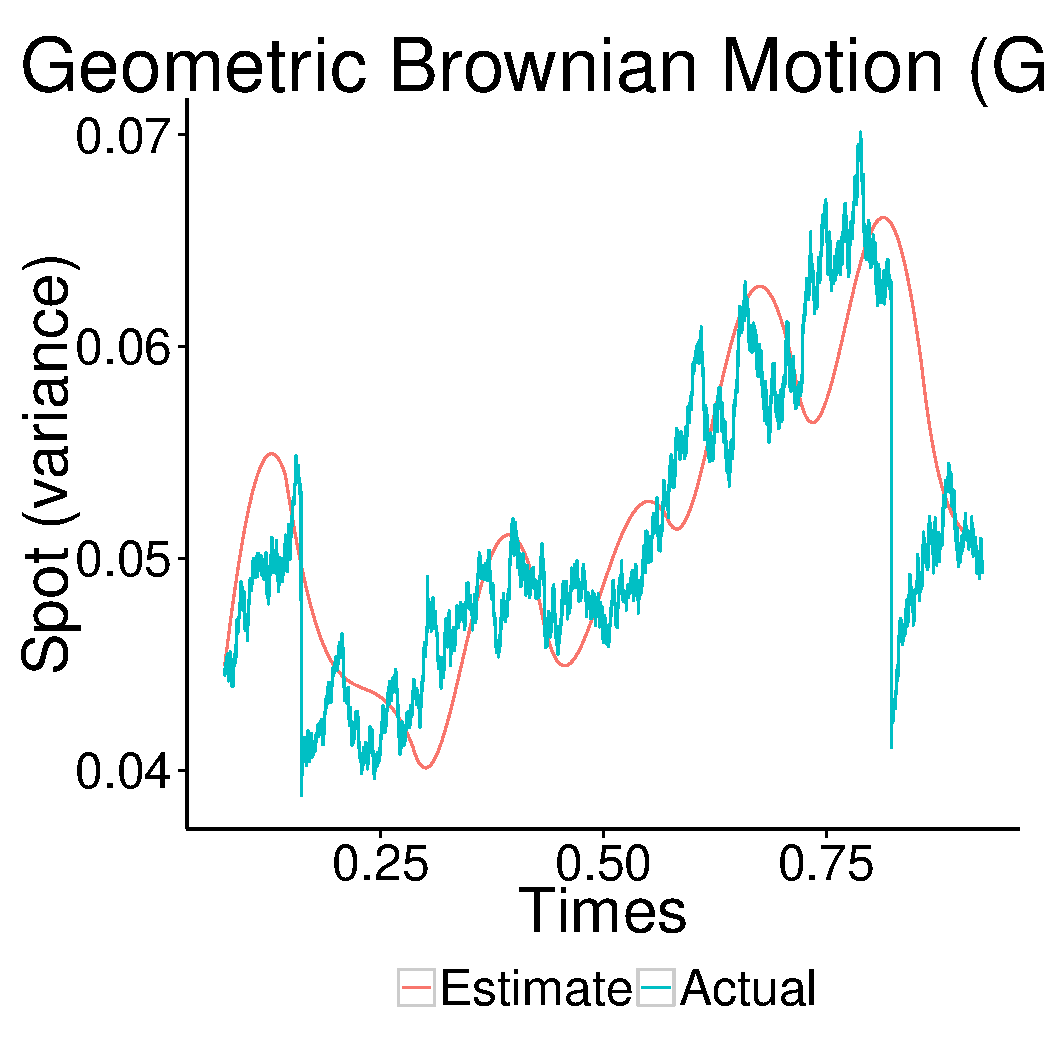
\includegraphics[width=0.45\textwidth]{/home/wale/Dropbox/Research/Paper3/pg.pdf}}}
  \quad
  \subfloat[CIR]{{ \includegraphics[width=0.45\textwidth]{/home/wale/Dropbox/Research/Paper3/pcir.pdf}}}
\quad
  \subfloat[OU]{{ 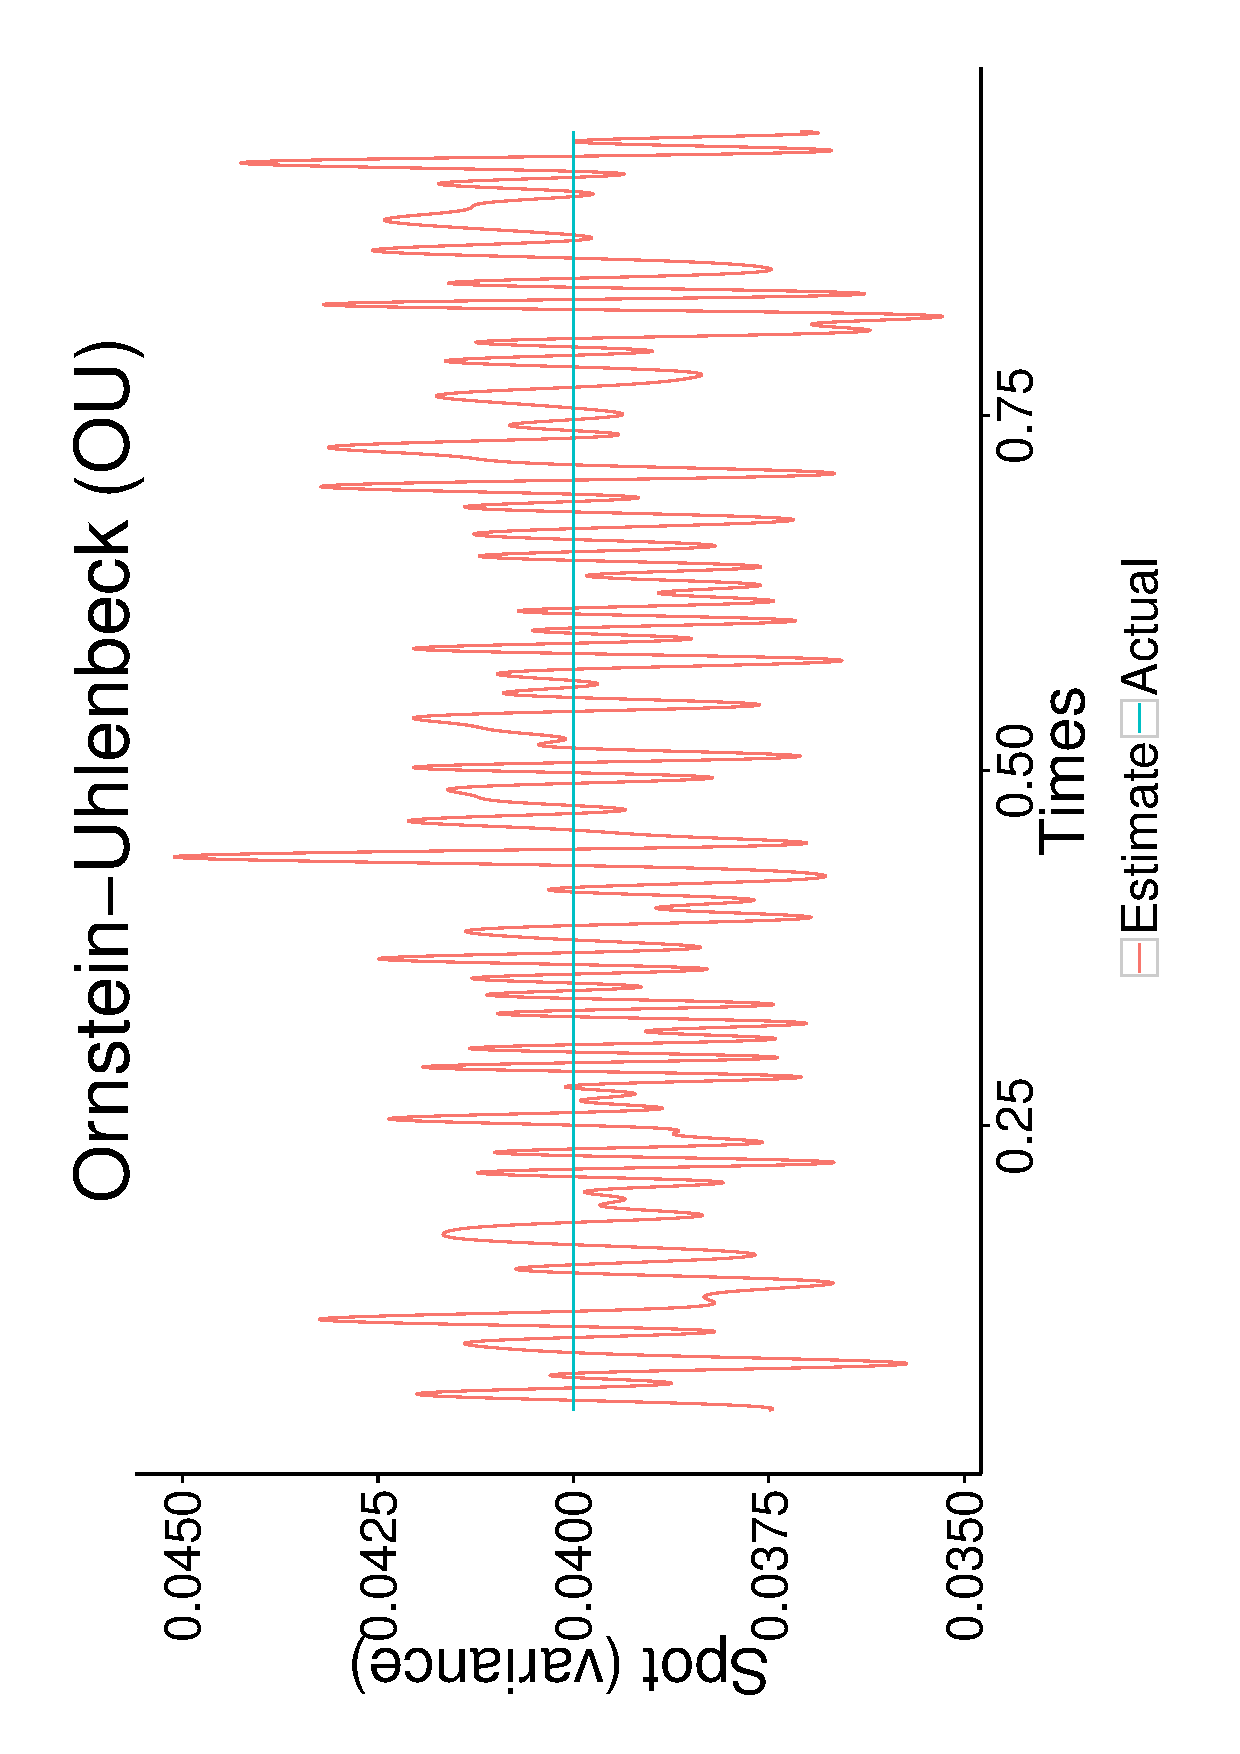
\includegraphics[width=0.45\textwidth]{/home/wale/Dropbox/Research/Paper3/po.pdf}}}
  \quad
  \subfloat[ABM]{{ \includegraphics[width=0.45\textwidth]{/home/wale/Dropbox/Research/Paper3/pa.pdf}}}
    \label{fig:path}
\end{figure}
\begin{comment}
  \end{comment}

  \framebreak
\begin{theorem} \label{pr:consistency}
  Let $\{g, \tilde{g}\}$ be pair of dual Gabor generators. If $g$ is Lipschitz continuous and  
  \begin{align}
    H_n^2 \Delta_n  + H_n^{-\alpha} \log H_n= o(1) \notag
    \label{}
  \end{align}
   then $R_n(\alpha,c)$ converges to 0, with 
  \begin{align}
    & B_n^2(\alpha,c)  = O(H_n^2\Delta_n  + H_n^{-2\alpha} \log^2 H_n)\notag \\
    & V_n(\alpha,c)  = O(H_n^2 \Delta_n), \notag
    \label{}
  \end{align}
  where  $\Delta_n = 1/n$ is the step size, and $H_n$ is the order of magnitude of the number of estimated frame coefficients. 
\end{theorem}
\end{frame}
\begin{frame}
  \frametitle{Future work}
  \begin{enumerate}
    \item cadlag volatility instead of just continuous volatility
    \item Price processes with jumps
    \begin{align}
      X_t = X_0 + \int_0^t \mu(s) d s + \int_0^t \sigma(s) d W_s + J_s, \qquad \forall t \ge 0\notag
      \label{}
    \end{align}
  \item Multivariate extension
  \item Emprirical study of spot volatility in fixed income markets
  \end{enumerate}
\end{frame}
\frame{
\section*{Market microstructure noise and spot volatility estimation}
\sectionpage
}
\begin{frame}[allowframebreaks]
  \frametitle{Market microstructure noise}
%\subsection{What is market microstructure}
\begin{enumerate}
  \item Noise generated from the moment-to-moment aggregate exchange behavior. The main sources of noise are:
    \begin{enumerate}
      \item \emph{The bid-ask spread}. The price at which an investor can buy an asset, at any fixed point in time,   is almost always greater than the price at which he may sell the asset. The \emph{real} or efficient price of the asset is somewhere in between (in most cases, it could be outside the range if there is private information not available to the other participants in the market)
      \item \emph{The price impact of trade}. The idea is that each transation releases information about the underlying asset. For instance, a buyer initiated transaction tells the market that the asset is more valuable than its current price to somebody. Now a really big buy transaction tells the market that someone with a lot of money and no doubt very sophisticated thinks the asset is more valuable than its currect. This can lead to the market overbidding the price of the asset even the foundamentals of the asset may not have changed.
      \item \emph{Price round-off} Say the market valuation of IBM stock is CHF 19.95666. Because markets prices are quoted up to a certain decimal place, the stock may be transacted at say CHF 19.95. In practice, this seems errelevant, but poses a big problem on any statistical procedure that assumes anything resembling \emph{recurrence or mixing}. This means that any possible value in the continuous range of our price will eventually show up in the data, given enough time. With rounding only numbers up to 2 decimal places will ever show up in our data. The vast majority of data having more than two decimal places will \emph{never} show up.
      \item{Human error} Especially, in the days of physical trrading pits quote were frequently misentered.
\end{enumerate}
\end{enumerate}
\end{frame}
\begin{frame}[allowframebreaks]
\frametitle{Why care about microstructure noise}
Short answer: It makes our statistical tools \emph{very, very inaccurate}. It also turns the world upside down. For example the more data you have the more inacurrate your estimate!
Consider the following:
\begin{align}
  Y_{t_i} = X_{t_i} + \varepsilon_{t_i},
\end{align}
where
\begin{align}
  X_t = x + \int_0^t \mu(s) ds + \int_0^t \sigma(s) d W_s \label{x}
\end{align}
and $W_s$ is a Brownian motion and $\varepsilon$ is independent of $X$.
The following is the coefficient associated with the Gabor frame expansion.
\begin{align}
  c_{h,k} = \int_0^1\overline{g_{h,k}(s)}\sigma(s)^2ds
\end{align}
A consiquence of the result from section 1 is that
\begin{align}
  \sum_{i=0}^{N} \overline{g_{h,k}(t_i)}(X_{{i+1}} - X_i)^2 & =    \int_0^1\overline{g_{h,k}(s)}\sigma(s)^2ds + o(1) \notag \\ 
  & (MISE)\notag
\end{align}
This works perfect without microstructure noise. With microstructure noise which in real markets is present, we have 
\begin{align}
  \sum_{i=0}^{N} \overline{g_{h,k}(t_i)}(Y_{{i+1}} - Y_i)^2& =    \int_0^1\overline{g_{h,k}(s)}\sigma(s)^2ds + 2N\omega^2_\varepsilon + o(1)\notag \\
  &(MISE) \notag
\end{align}
%where $Y_{t_i} $ is the observed noisy price, $X_{t_i}$ is the efficient price, and $\varepsilon_{t_i}$ is a model for market microstructure noise.
\end{frame}
\begin{frame}
  \frametitle{Two-time scales/subsampling}
  We adapt the two timescales approach of Zhang et al. (2005) to obtain consistent coefficient estimates.
 
\begin{align}
  &\hat{\sigma}^2_n(t) = \sum_{h,k} c_{h,k}^b\;g_{h,k}(t),\qquad \forall t \in [0,T], \label{eq:noiseest}
\end{align}
where
\begin{align}
  &c_{h,k}^b = c_{h,k}^R - (m_n/n)c_{h,k} \\
  &c_{h,k}^R = (1/R_n)\sum_{i =0}^{n -R_n} \overline{g_{h,k}(t_i)} (Y_{t_{i+R_n}} - Y_{t_i})^2 \label{eq:subset} \\
  &c_{h,k} = \sum_{i =0}^{n-1} \overline{g_{h,k}(t_i)} (Y_{t_{i+1}} - Y_{t_i})^2.
  \label{}
\end{align}
\end{frame}
\begin{frame}
  \frametitle{Future work}
  \begin{enumerate}
    \item Rigurous proof 
    \item Extension to Ito semimartingale. Jumps, cadlag volatility.
    \item Simulation study
    \item Empirical study
  \end{enumerate}
\end{frame}
%------------------------------------------------
\frame{
\section*{Tracking changes in bond market stability}
\sectionpage
}
\begin{frame}
  \frametitle{The empirical evidence}
  \begin{enumerate}
    \item 
  Litterman \& Scheinkman (1991). 98\% Volatility of spot short rate acconted for by three factors. 89\% for the first component. 
\item Bouchaud et al. (1999) report a decay rate faster than $q^{-4}$, where $q$ is the rank of the component.
  \end{enumerate}
\end{frame}
\begin{frame}
  \frametitle{The HJM model of fixed income markets}
  Models the entire forward rate curve (FRC). The FRC is a stochastic ``curve''.For each maturity $\tau$, we have
  \begin{align}
    &f(t, \tau) = f(0, \tau) + \int^t_0\mu(s,\tau) d s + \int^t_0\sum^m\sigma_j(s,\tau)d W_j(s),\notag
    \label{}
  \end{align}
which is the instantanious return on a loan contracted at time $t$ for issue at time $\tau$. 
\end{frame}
\begin{frame}
  \frametitle{Realized Spectrum}
  The empirical evidence suggests there is $d \approx 3$ such  that  the co-volatility matrix of the foreward rates satisfies
  \begin{align}
    &\Sigma(t) \approx \sum^d_i \lambda_i(t) (v_i(t) \otimes v_i(t))
    \notag
    \label{}
  \end{align}
 where $\lambda_i(t)$ and $v_i(t)$ are the $i$-th most principal eigen value and eigenvector of $\Sigma(t)$. 
 We propose to estimate the spectrum of $\Sigma(t)$ via the spectrum of $\hat{\Sigma}(t)$, the Gabor frame estimate of the covolatility matrix. So that
 \begin{align}
   &\hat{\Sigma}(t) \approx \sum^d_i \hat{\lambda}_i(t) (\hat{v}_i(t) \otimes \hat{v}_i(t))
    \notag
    \label{}
  \end{align}
\end{frame}
\begin{frame}
  \frametitle{Tracking and predicting market swings}
  The first eigen vector has been found to be very stable, fluctuating only during periods of market turmoil. (Carmona \& Tehranchi (2006)) It does makes sense to monitor changes in the first eigen vector. This can be summarized conveniently using consines:
  \begin{align}
    \chi_1(t_i) = \frac{\langle \hat{v}_1(t_i), \hat{v}_1(t_{i-1})\rangle}{\Vert \hat{v}_1(t_i)\Vert \Vert \hat{v}_1(t_{i-1})\Vert}\notag
    \label{}
  \end{align}
 Does  $\chi_1(t_i)$ contain leading information about foreward rates?
\begin{align}
  f(t_i, \tau) = \alpha_{\tau} + \sum_{j=1}^q\beta_{\tau,j} \hat{\chi}_{n,1} (t_{i-j}) + \sum_{j=1}^p\gamma_{\tau,j} f(t_{i-j},\tau)+ \eta_{\tau,i},
  \label{}
\end{align}
\end{frame}
\end{document} 
